\section{Основы линейной и нелинейной оптики.}

\subsection{Материальное уравнение линейной среды.}
\hspace*{2mm}
В основе взаимодействия света со средой лежит элементарный процесс возбуждения атома или молекулы вещества световым полем и последующего переизлучения света возбужденной частицей. Характер этого взаимодействия зависит от соотношения между величиной напряженности поля световой волны Е и характерной напряженностью внутриатомного поля  $E_{atom}$, определяющего силы связи оптических электронов (т.е. внешних, наиболее слабо связанных электронов) с ядром атома вещества.
\\
\hspace*{2mm}
Например, для атома водорода это поле составляет $ E_{atom} = e/(4\pi\epsilon_{0}r_{h}^2) = 5\cdot10^{11} $В/м, для более тяжелых атомов $ E_{atom} = 10^{10} \dots 10^{11} $ В/м. Оценка поля Е световой волны в случае не лазерных источников свет дает величину $E \le 10^3$ В/м, т.е. $E<<E_{atom} $. При этом условии отклик атомного осциллятора на внешнее воздействие будет иметь линейный характер, а зависимость поляризованности Р = Р(Е) в случае изотропной среды может быть представлена в виде:
\begin{equation}\label{1:liner}
P(E) = \chi^{(1)}E
\end{equation}

где $ \chi^{(1)}$ – линейная восприимчивость среды, являющаяся безразмерной величиной и зависящая только от свойств среды.
Материальное уравнение ($\ref{1:liner}$) является одним из соотношений, на которых базируется линейная оптика.  Но оно справедливо только при условии $E << E_{atom} $, а во слех остальных случаях является лишь некоторым приближением. 
\\
В мощных лазерных пучках можно получить напряженности уже сравнимые с $E_{atom} $. В случае когда поле Е, оставаясь меньше $E_{atom} $, приближается к нему по величине, поляризованность среды Р = Р(Е) перестает быть линейной функцией поля Е, и в этом случае материальное уравнение ($\ref{1:liner}$) должно быть заменено на другое.

\subsection{Материальное уравнение нелинейной среды.} 
\hspace*{2mm}
Теория нелинейно-оптических явлений строится на основе материальных уравнений и уравнений Максвелла. Уравнения Максвелла для диэлектрической нейтральной немагнитной среды имеют вид
\begin{equation}\label{1:maxvel}
rot\vec{E} = - \frac{ 1 }{ c}\frac{\partial \vec{H} }{\partial t}
\hspace{20mm}
rot\vec{H} =  \frac{ 1 }{ c}\frac{\partial \vec{D} }{\partial t}
\hspace{20mm}
div\vec{H} = 0
\end{equation}
где $ \vec{D} = \vec{E} + 4\pi \vec{P}$. Из уравнений Максвелла вытекает волновое уравнение
\begin{equation}\label{1:rot_maxvel}
rot(rot\vec{E}) + \frac{ 1 }{ c^2 }\frac{\partial^2 \vec{E} }{\partial t^2} = - \frac{ 4\pi }{ c^2 }\frac{\partial^2 \vec{P} }{\partial t^2}
\end{equation}
которе в случае изотропной среды принимает вид
\begin{equation}\label{1:wave_eq}
\Delta\vec{E} - \frac{ 1 }{ c^2 }\frac{\partial^2 \vec{E} }{\partial t^2} =  \frac{ 4\pi }{ c^2 }\frac{\partial^2 \vec{P} }{\partial t^2}
\end{equation}
где $\vec{E}$ - напряженность электрического поля, а $\vec{P}$ - поляризация среды. Поляризация среды возникает под действием падающий световой волны и описывается материальным уравнением $\vec{P} = \vec{P}(\vec{E})$.
В анизотропном случае $\vec{P}(\vec{E})$ являеться тензорный величиной и может быть представлена в виде:
\begin{equation}\label{1:p_1}
P(E) = \chi^{(1)}E + \chi^{(2)}E^2 \chi^{(3)}E^3\dots
\end{equation}
Коэффициенты $\chi^{(m)}, m \ge 2$ при членах разложения называются нелинейными восприимчивостями m-го порядка и являются уже размерными величинами. При этом соответствующая величина $\chi^{(m)}$ пропорциональна концентрации атомов (молекул) в веществе и m-ой степени параметра. Это означает, что отклик среды на действие внешнего светового поля перестает быть линейным.  С математической точки зрения именно это обстоятельство (нелинейность материального уравнения) является причиной нарушения принципа суперпозиции для световых волн в нелинейной среде. Из уравнений (\ref{1:rot_maxvel}), (\ref{1:wave_eq}) и (\ref{1:p_1}) непосредственно вытекает возможность генерации оптических гармоник и других нелинейно-оптических эффектов.  Надо отметить, что среды, в которых достаточно учитывать только первых два члена в уравнении ($\ref{1:wave_eq}$), называют квадратично-нелинейными средами, а среды с тремя первыми членами - кубически-нелинейными. 

\subsection{Нелинейная поляризация.} 
\hspace*{2mm}
Часть поляризации среды, нелинейно зависящая от напряженности светового поля, называется нелинейной поляризацией.Выделяя в поляризации среды линейную и нелинейную компоненты, можно записать:
\begin{equation}\label{1:p_non_liner}
\vec{P} = \vec{P}_{liner} + \vec{P}_{nonliner}
\end{equation}
подставив уравнение  (\ref{1:p_non_liner}) в  (\ref{1:rot_maxvel}) получим волновое уравнение для анизотропной среды и нелинейной изотропной среды:
\begin{equation}\label{1:wave_eq2}
\Delta\vec{E} - \frac{ 1 }{ c^2 }\frac{\partial^2 \vec{E} }{\partial t^2} - \frac{ 4\pi }{ c^2 }\frac{\partial^2 \vec{P}_{liner}}{\partial t^2} =  \frac{ 4\pi }{ c^2 }\frac{\partial^2 \vec{P} _{nonliner}}{\partial t^2}
\end{equation}
Нелинейная поляризация среды является источником новых спектральных компонент поля (оптических гармоник, комбинационных частот и т. п.). Материальное уравнение вида  (\ref{1:wave_eq}), описывает изотропную нелинейную среду с безынерционным локальным откликом на световое поле. Аналогичное уравнение для анизотропной нелинейной диспергирующей среды является уже не только тензорным, но и имеет комплексную часть: 
\begin{equation}
\chi^{(m)} = Re(\chi^{(m)}) + iIm(\chi^{(m)})
\end{equation}
причем коэффициенты восприимчивости, входящие в данное уравнение, уже зависят от времени о координаты. Среды, обладающие таким свойством, называют средами с пространственной дисперсией. К их 
числу относятся некоторые типы кристаллов, а также плазма.

\subsection{Основные процессы и эффекты нелинейной оптики}
Физические причины, приводящие к появлению нелинейных оптических эффектов, достаточно многообразны. К ним можно отнести:
\begin{enumerate}
\item  Нелинейную рефракцию в оптически прозрачной среде, т.е. зависимость показателя преломления среды от амплитуды светового вектора;
\item  Нелинейный характер рассеяния света в среде при больших интенсивностях светового поля;
\item  Многофотонное поглощение интенсивного оптического излучения в веществе;
\item  Генерацию высших гармоник при переизлучении световой волны;
\item  Тепловые самовоздействия и др.
\end{enumerate}
\begin{figure}[h]
	\centering
	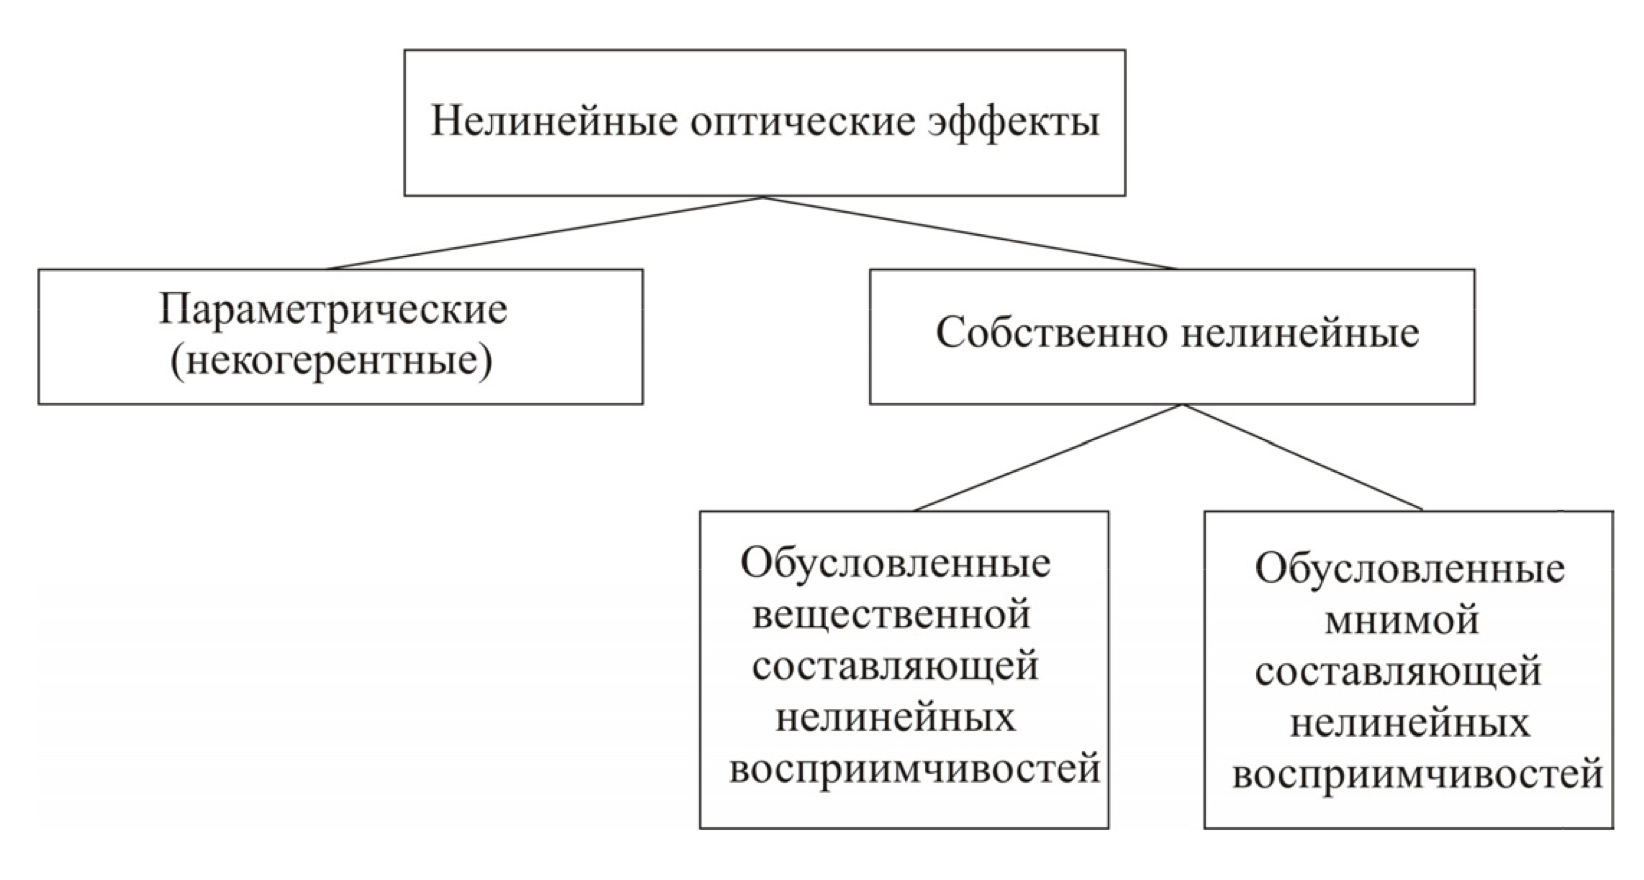
\includegraphics[width=0.7\linewidth]{images/classific.png}
	\caption{Классификация нелинейных оптических эффектов}
	\label{classific}
\end{figure}
К \textit{параметрическим явлениям} относятся:
\begin{enumerate}
\item   Электрооптический эффект, или эффект Поккельса (сообщение оптической анизотропии кристаллическим изотропным диэлектрикам без центра инверсии, помещенным в сильное однородное электрическое поле, при этом показатель преломления становится нелинейной функцией напряженности поля); является нелинейным эффектом второго порядка;
\item Эффект Керра (аналогичен эффекту Поккельса, но является нелинейным эффектом третьего порядка) и ряд других.
\end{enumerate}
К эффектам, \textit{обусловленным вещественной составляющей нелинейных восприимчивостей}, относятся:
\begin{enumerate}
\item  Эффекты генерации высших оптических гармоник, в частности, связанные с удвоением и утроением частоты света;
\item  Самовоздействие интенсивного светового пучка в нелинейных материалах (например, явление самофокусировки, при котором возникает перепад свойств среды в пучке и вне пучка, а его распространение приобретает волноводный, нитевидный характер, устраняющий геометрическую и дифракционную расходимость; при самофокусировке нарушается закон прямолинейного распространения света);
\item Оптический пробой среды, в основе которого лежит процесс качественного превращения прозрачной в сильно поглощающую среду с изменением агрегатного состояния при некотором значении интенсивности света;
\end{enumerate}
К эффектам, \textit{обусловленным мнимой составляющей нелинейных восприимчивостей}, относятся:
\begin{enumerate}
\item  Многофотонные процессы (фотоионизация и фотовозбуждение, гиперрассеяние света и другие), когда в элементарном акте взаимодействия света с атомом вещества участвует не один, а несколько фотонов; если мнимая составляющая линейной восприимчивости ответственна за однофотонные процессы, то мнимые составляющие восприимчивостей высших порядков – за многофотонные процессы;
\item  Вынужденное комбинационное рассеяние света, заключающееся в том, что интенсивное падающее излучение вызывает появление в оптической среде волны рассеянного стимулированного излучения на смещенных (комбинационных) частотах, характеристики которого имеют нелинейную зависимость от характеристик вынуждающего излучения;
\item Вынужденное рассеяние Мандельштама – Бриллюэна, при котором мощное световое излучение возбуждает в среде когерентные колебания молекул по закону бегущей волны, при этом происходит рассеяние света на образовавшейся периодической структуре (сверхзвуковой волне).
\end{enumerate}

\subsection*{Многофотонное поглощение}
В процессе многофотонного поглощения атом переходит из основного состояния в возбужденное при одновременном поглощении двух и более фотонов. При этом сечение поглощения (отношение мощности поглощенного излучения к интенсивности падающей волны), в отличие от сечения «обычного», линейного поглощения, зависит от интенсивности. Например, для двухфотонного поглощения,
\begin{equation}\label{2photon}
\sigma = \sigma^{(2)}I
\end{equation}
Следовательно, скорость перехода зависит от интенсивности квадратично:
\begin{equation}\label{2photon1}
R = \frac{\sigma I}{ \hslash \omega } =  \frac{\sigma^{(2)}I^{(2)}}{\hslash\omega}
\end{equation}
Двухфотонное поглощение – полезный спектроскопический метод для определения положения атомных уровней, которые не связаны с основным состоянием однофотонными переходами.

\subsection*{Вынужденное рассеяние}
Вынужденное рассеяние отличается от спонтанного тем, что падающее лазерное излучение, интерферируя с рассеянной волной, «раскачивает» неоднородности среды, на которых происходит рассеяние. Поэтому интенсивность вынужденного рассеяния может быть намного порядков больше, чем спонтанного. Примеры вынужденного рассеяния: комбинационное (ВКР) – рассеяние на колебаниях молекул среды, Мандельштама-Бриллюэна (ВРМБ) – на флуктуациях плотности (фононах), рэлеевское, и т. д.
\\
На основе процессов вынужденного рассеяния можно создавать лазеры (например, распространены рамановские лазеры на ВКР). При определѐнных условиях при вынужденном рассеянии наблюдается интересный эффект – обращение волнового фронта.

\subsection*{Генерация второй оптической гармоники} 
\hspace{2mm}
Обсудим подробнее эффект удвоения частоты света в кристалле — генерации второй оптической гармоники. Данный эффект состоит в том, что под действием мощного лазерного излучения в нелинейном кристалле возникает излучение на удвоенной частоте.
\\
\hspace{2mm}
Пусть на квадратично-нелинейную среду воздействует монохроматическое поле с частотой $\omega$:
\begin{equation}\label{shg:e(t)}
A(t) = A\cos(\omega t)
\end{equation}
Тогда нелинейная поляризация второго порядка будет пропорциональна полю во второй степени:
\begin{equation}\label{shg}
P(t)^{(2)} = \chi^{(1)}E(t)^2 = \frac{1}{2}\chi^{(1)}A^2 + \frac{1}{2}\chi^{(1)}A^2\cos(2\omega t)
\end{equation}
Это значит, что поляризация будет иметь постоянную составляющую $ \frac{1}{2}\chi^{(1)}A^2$ , и переменную $\frac{1}{2}\chi^{(1)}A^2\cos(2\omega t)$, на удвоенной частоте $2\omega$. Первое слагаемое в (\ref{shg}) соответствует нелинейному процессу, который называется \textbf{оптическим выпрямлением}, а второе – \textbf{генерации второй гармоники}. 
\\
Происходит возбуждение волны поляризации на удвоенных частотах $2\omega_{1,2}$ (\textbf{генерация второй гармоники}, SGH), разностной $\omega_1 + \omega_2$(\textbf{генерация разностной частоты}, ГРЧ), суммарной $\omega_1 - \omega_2$ (\textbf{генерация суммарной частоты}, ГСЧ), и нулевой (\textbf{оптическое выпрямление}) частотах (рис. \ref{sghPictr}).
\begin{figure}[h]
	\centering
	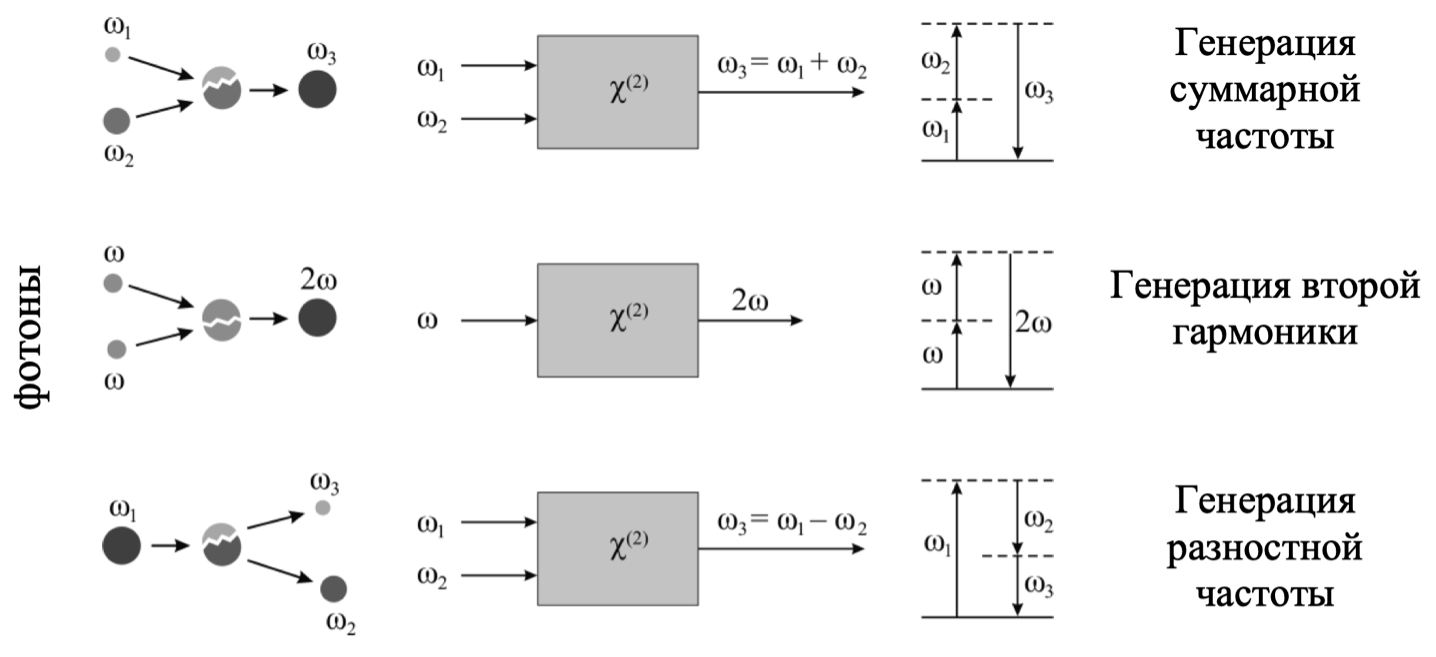
\includegraphics[width=0.7\linewidth]{images/shg.png}
	\caption{Схематическое представление нелинейно-оптических процессов второго порядка.}
	\label{sghPictr}
\end{figure}

\subsection*{Генерация третей оптической гармоники} 
Пусть на квадратично-нелинейную среду воздействует монохроматическое поле (\ref{shg:e(t)}) с частотой $\omega$. Тогда поляризация третьего порядка зависит от времени следующим образом:
\begin{equation}\label{thg}
P(t)^{(3)} = \chi^{(3)}E(t)^3 = \frac{1}{4}\chi^{(3)}A^3\cos(3\omega t) + \frac{3}{4}\chi^{(3)}A^3\cos(\omega t)
\end{equation}
То есть, происходит генерация третьей гармоники (THG) и переизлучение на исходной частоте (\textbf{самовоздействие света}) – см. рис. \ref{thg1}A, B. Поскольку, как правило, $\chi^{(3)}E^3 << \chi^{(2)}E^2$ то эффект THG в кубически-нелинейной среде очень мал, и на практике третью гармонику лазерного излучения получают путѐм последовательного удвоения частоты $\omega +  \omega \rightarrow 2\omega$, а затем сложения волн первой и второй гармоники: $\omega +  2\omega \rightarrow 3\omega$ в квадратично-нелинейной среде
\begin{figure}[h]
	\centering
	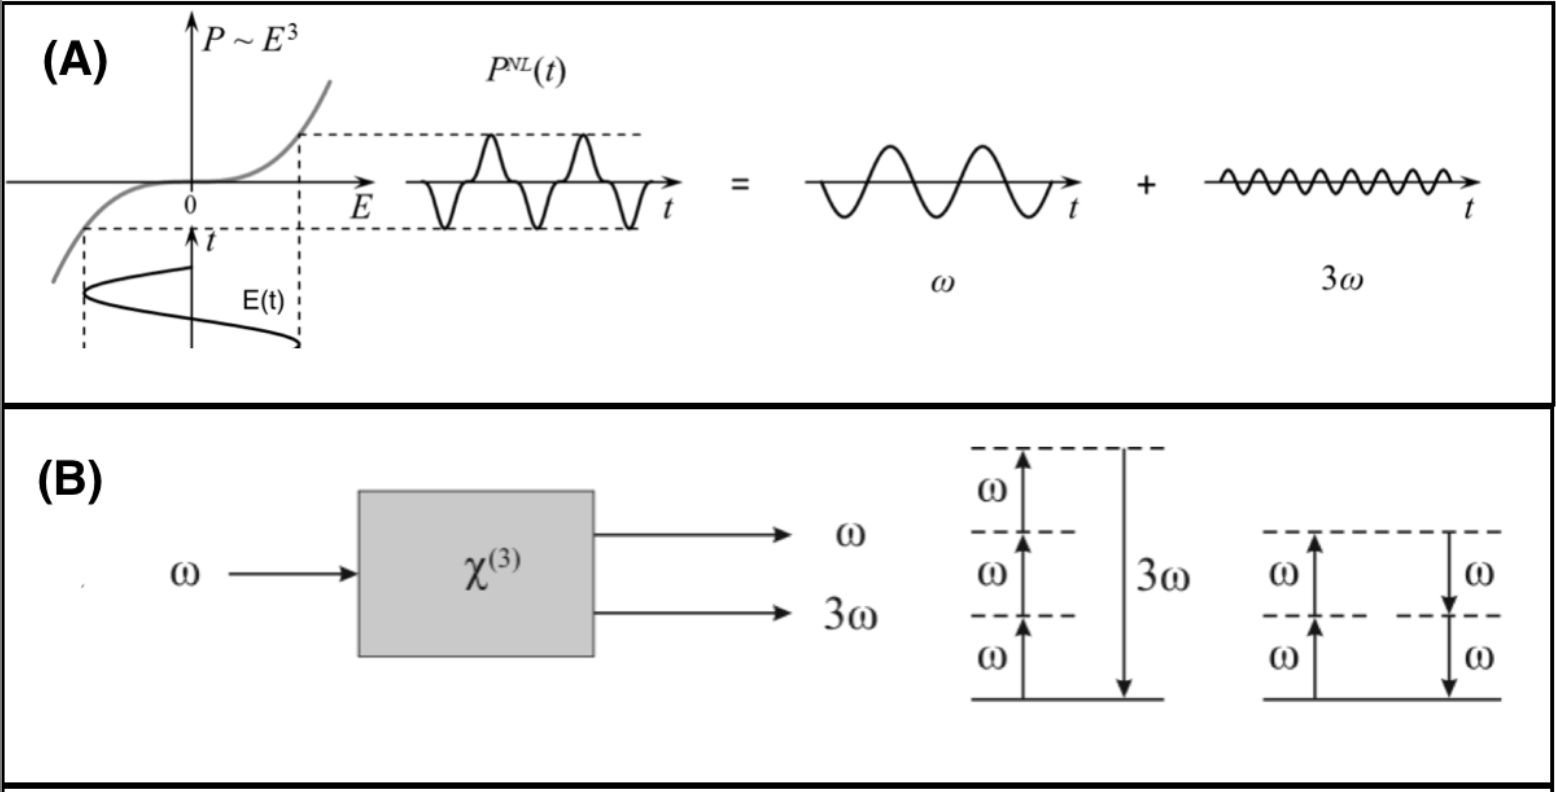
\includegraphics[width=0.8\linewidth]{images/thg.png}
	\caption{\textbf{(A)}: Поляризация среды третьего порядка. \textbf{(B-D)}: Схематическое представление нелинейнооптических процессов третьего порядка.}
	\label{thg1}
\end{figure}
В общем случае следует рассматривать оптическое поле как сумму трех волн: $E(t) = \frac{1}{2}(A_1e^{i\omega_1 t} + A_2e^{i\omega_2 t} + A_3e^{i\omega_3 t})$. Тогда будут возбуждаться колебания поляризации на всевозможных кобинациях частотат (пример некоторых процессовт рис. \ref{thg1}B-D, так-же см. ниже частотный смеситель\ref{mixerPictr1}). Второе слагаемое в правой части уравнения (\ref{thg}) описывает самовоздействие света. В простейшем случае можно показать, что оно сводится к изменению показателя преломления пропорционально интенсивности света: $n = n_0 + \gamma I$, где $ \gamma = \frac{12\pi^2 \chi^{(3)}}{n_{0}^{2}c} $. Если нелинейный коэффициент $\gamma > 0$, то показатель преломления в центре пучка, где интенсивность максимальна, больше, чем на периферии, поэтому пучок сходится к оси. Этот процесс называется \textbf{самофокусировкой}. В противном случае, при $\gamma < 0$, происходит \textbf{самодефокусировка} излучения. 